\chapter{Przetwarzanie heterogeniczne}\label{cha:hpo}

%---------------------------------------------------------------------------

\section{Wprowadzenie}\label{sec:wprowadzenie}


Lata 50-te XX wieku były przełomowym okresem w dziedzinie elektronicznego przetwarzania danych. Opracowana w 1945 roku Architekura von Neumana [16] pozwoliła na uruchomienie pierwszych komputerów ogólnego przeznaczenia. Mimo, że Architektura Harwardzka [17] została opracowana 6 lat wcześniej, Architektura von Neumana była łatwiejsza w implementacji przez przechowywanie danych wraz z programem na jednej wspólnej pamięci. Pierwszym komputerem opartym na pomyśle Neumana, który wykonywał instrukcje zapisane w fizycznej pamięci , był powstały w 1948 roku Small-Scale Experimental Machine. Był on bazą do rozwijania kolejnych urządzeń i tak w 1949 roku powstał EDSAC (akronim od ang. Electronic Delay Storage Automatic Calculator). Został uznany jako  pierwszy komputer wykorzystywany w praktyce do obliczeń naukowych. EDSAC rozbudowany był o dodatkowe układy peryferyjne. W celu odczytu danych zastosowano w nim dalekopis – aparat drukujący dane w postaci alfanumerycznej. Skonstruowanie komputerów zerowej, pierwszej i drugiej generacji znacznie rozwinęło moc obliczeniową tych urządzeń. W dalszym ciągu jednak stosowano niewygodne formy prezentacji danych – wyświetlacze złożone z szeregu lamp, perforowane karty. W 1975 roku, w jednym z pierwszych komputerów osobistych IBM 5100, zastosowano kineskopowy wyświetlacz, który mógł wyświetlać 16 linii po 64 znaków. 6 lat później , w kolejnym modelu IBM 5150, wprowadzono możliwość instalacji kart rozszerzeń ISA. Zastosowano w nim pierwszą kartę graficzną Monochrome Display Adapter (MDA). Rozpoczęło to rozwój peryferyjnych układów komputera, które stały się niezależnymi platformami z własnym procesorem i pamięcią. Początkowo karty graficzne były w stanie wyświetlać jedynie znaki alfanumeryczne przechowywane w pamięci karty. Kolejne generacje kart pozwalały na rysowanie obrazów przy użyciu pojedynczych pikseli, a nowoczesne układy graficzne pozwalały na akcelerację 2D i 3D, korzystając z wbudowanych funkcji do generowania obrazu. W najnowszych procesorach grafiki umożliwiono użytkownikowi zaprogramowanie ich w dowolny sposób. Charakterystyka obliczeń przy przetwarzaniu obrazów wymusiła architekturę procesorów graficznych w postaci dużej ilości jednakowych jednostek ALU (ang. Arithmetic Logic Units), potrafiących wykonać równolegle wiele prostych operacji (Rys. 3.1.).
\begin{figure}[h]
        \centering
                \centering
                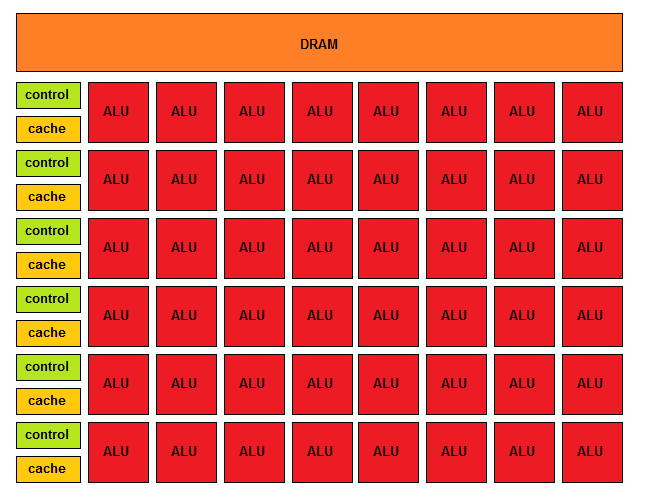
\includegraphics[width=12cm]{rys7}
	\caption{Architektura procesora GPU.}
\end{figure}
Taka budowa kart graficznych pozwoliła na wykorzystanie ich nie tylko do obliczeń związanych z generowaniem grafiki, ale także innych obliczeń przetwarzania danych , co doprowadziło do powstania kart ogólnego przeznaczenia (GPGPU).



%---------------------------------------------------------------------------

\section{Heterogeniczne platformy obliczeniowe}\label{sec:hetero}

Początkowo GPGPU były wykorzystywane do zaawansowanego generowania grafiki. Dążenie do realizmu w grach komputerowych rozwinęło karty graficzne o algorytmy wymagające przetwarzania równoległego, takie jak shading [18] czy ray-tracing [19]. W celu odciążenia procesora od złożonych obliczeń, na kartach graficznych zaczęto implementować fizykę obiektów – obliczenia związane z mechaniką klasyczną, symulacje zachowania cieczy, zachowania układów ciągłych i inne efekty cząsteczkowe. Dla ułatwienia programistom wykorzystania możliwości GPGPU, NVIDIA w 2007 roku wprowadza platformę CUDA. Jest to środowisko programistyczne i biblioteka umożliwiająca wykorzystanie kart graficznych produkowanych przez firmę NVIDIA. Umożliwia ona pisanie kodu opartego na C/C++ wykonywanego na procesorze karty i mającego bezpośredni dostęp do jej pamięci. Ułatwienie implementacji algorytmów na GPGPU rozwinęło wykorzystywanie tych kart w różnych dziedzinach naukowych, takich jak kryptografia, fizyka kwantowa, ekonomia czy medycyna. Wykonywanie  skomplikowanych obliczeń przy użyciu CUDA stało się powszechne na komputerach domowych, ale było ograniczone przez wymagania sprzętowe. 2 lata po wprowadzeniu CUDA firma Apple Inc wprowadza OpenCL (ang. Open Computing Language). W przeciwieństwie do produktu NVIDA, OpenCL umożliwia pisanie programów na heterogeniczne platformy – układy złożone z różnego rodzaju procesorów. Daje to możliwość pisania aplikacji na komputery z układami większości popularnych producentów, lub dowolne układy złożone z różnych procesorów (m. in. CPU, GPU, DSP, FPGA), oraz zapewnia przenośność programów.

%---------------------------------------------------------------------------

\section{Środowisko OpenCL}\label{sec:OpenCL}

OpenCL jest platformą programistyczną opracowaną w 2009 roku przez Apple Inc, a następnie utrzymywaną przez Khronos Group. Umożliwia programowanie heterogenicznych układów procesorowych w języku opartym na C99 i C++11.


Aplikacja pisana w OpenCL opiera się na jednostkach zwanych platformami. Każda platforma odpowiada za przygotowanie danych do obliczeń i rozdzieleniem zadań. W nowszych standardach kod platformy może być pisany w wielu popularnych językach  (m. in. Python, Matlab). Każda platforma zawiera kontekst, w którym definiowane są dane wejściowe, kolejka zadań i urządzenia do wykonywania obliczeń. Każde urządzenie zawiera jednostki obliczeniowe (ang. compute units, CU), które składają się z elementów przetwarzania (ang. processing elements, PEs)(Rys. 3.2.). 

\begin{figure}[h]
        \centering
                \centering
                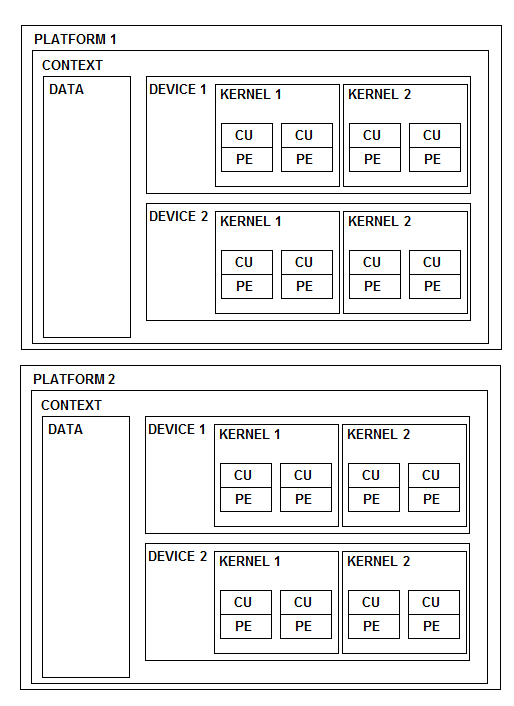
\includegraphics[width=12cm]{rys8}
	\caption{Architektura programu napisanego w bibliotece OpenCL.}
\end{figure}

Elementy przetwarzania wykonują specjalnie przygotowane funkcje (tzw. kernele), definiowane według standardu OpenCL. W zależności od urządzenia (karta graficzna, procesor itp.), CU i PE reprezentują różne elementy procesora, ale odwołuje się do nich w ten sam sposób. Umożliwia to wykonywanie  kernela o jednakowej składni na różnych typach procesorów. Kernele wykonywane są według kolejki zadań i rozdzielone pomiędzy jednostki obliczeniowe mogą być wykonywane równolegle na wielu elementach przetwarzania. Każda kolejka zadań definiuje przestrzeń indeksowania, w której wykonywane są poszczególne kernele.  Instancje kernela wywołaną w obrębie jednego indeksu nazywamy wątkiem. Przestrzeń indeksów można podzielić na grupy (ang. work-group), do których należą poszczególne wątki.


OpenCL umożliwia dynamiczny dostęp do pamięci urządzeń. Zdefiniowane są cztery typy pamięci:

- pamięć globalna – pamięć dostępna przez wszystkie wątki w obrębie jednego kontekstu

- pamięć stała – pamięć tylko do odczytu, dostępna globalnie

- pamięć lokalna – pamięć dostępna w obrębie jednej grupy wątków

- pamięć prywatna – pamięć dostępna w obrębie jednego wątku\\


 Przepływ danych między platformą  a urządzeniem może odbyć się poprzez operację kopiowania  lub odwzorowania z pamięci platformy do pamięci urządzenia.


Dużym ograniczeniem wydajności obliczeń jest czas dostępu do pamięci. Pamięć o szerszym zakresie ma wolniejszy czas dostępu, dlatego najwydajniejsze obliczeniawykonują się dla niezależnych wątków działających równolegle o prywatnej pamięci.















